\documentclass{article}

\PassOptionsToPackage{numbers,sort&compress}{natbib}
\usepackage[dblblindworkshop]{neurips_2026}
\workshoptitle{New in Machine Learning (NewInML) at NeurIPS 2026}

\usepackage[utf8]{inputenc}
\usepackage[T1]{fontenc}
\usepackage{hyperref}
\usepackage{url}
\usepackage{booktabs}
\usepackage{amsmath}
\usepackage{graphicx}
\usepackage{xcolor}
\usepackage{microtype}

% Auto-generated submission profile
\newif\ifincludeappendix
\includeappendixfalse


\title{Toward Mechanical Scientific Models: Fractal Custody and Governed Agent Experiments}

\author{Anonymous Author(s)}

\begin{document}

\maketitle

\begin{abstract}
The \emph{Mechanical Scientific Method} treats scientific computation as a sequence of governed state transitions in which evidence, transforms, and bounded claims remain inspectable rather than collapsed into model prose.
We propose the term \emph{Mechanical Scientific Model} for a computational model class that satisfies explicit requirements: explicit evidence state; governed and versioned state transitions; separation of deterministic transforms from probabilistic model outputs; preservation of positive, null, negative, failed, blocked, timeout, abstention, and contradictory outcomes; explicit claim ceilings; forward and reverse evidence traceability; and successor-state recording rather than silent history rewriting.
\emph{Fractal Custody Objects} (FCOs) and a \emph{Fractal Custody Graph} (FCG) provide the custody substrate for binding those transitions.
HydraDG is the primary experimentally evaluated implementation examined here: it preregisters hypotheses, freezes case manifests and scorers, records raw prompt and response hashes, and preserves terminal states without silent substitution.
We report two preregistered HydraDG studies (EXP-008, EXP-009) comparing flat prose versus structured FCG retrieval for failure-prevention endpoints; both terminate as \emph{underpowered}, so confirmatory treatment-effect claims are not supported while null, negative, and failure evidence remains in custody.
We do not claim that Mechanical Scientific Models are an established external field term; we offer them as a proposed model class and report bounded custody behavior from one implementation.
\end{abstract}

\section{Introduction}

Large language model agents are evaluated on task success, benchmark scores, and human preference \cite{liu2023agentbench,zhou2023webarena}.
Less often preserved are the conditions under which experiments fail: swapped models, stale runtime selection, partial matrix execution, or JSON outputs that never parse.
When negative and null cells disappear from the public record, later work cannot distinguish \emph{no effect} from \emph{no measurement}.

This paper separates five layers that are often conflated in agent-evaluation reporting:
\begin{itemize}
  \item \textbf{Method} --- the \emph{Mechanical Scientific Method}: governed transitions among explicit evidence states rather than narrative collapse of runs into conclusions.
  \item \textbf{Model class} --- \emph{Mechanical Scientific Models} (proposed here; not an established external terminology): computational systems whose state transitions are mechanically exposable and failure-complete.
  \item \textbf{Custody substrate} --- FCO/FCG receipts that bind source bytes, transforms, derived evidence, bounded claims, and successor state.
  \item \textbf{Primary implementation} --- HydraDG, the experimentally evaluated implementation whose preregistered EXP-008 and EXP-009 results are reported here.
  \item \textbf{Systems validation and companion exemplars} --- HydraLamp perturbation receipts and HydraDG scoring on local Apple Silicon (Mac Studio class, 32\,GB RAM); companion implementation lineages are excluded from primary inference for EXP-008/009 and are not part of the reviewed source set for this submission.
\end{itemize}

HydraDG instantiates the proposed model class through a custody-first experimental contract.
Every actor---human operator, frontier agent, local model runtime, or deterministic script---must emit or be represented by a handoff receipt before its output is promoted.
Receipts bind actor identity, host, repository state, input hashes, raw output hashes, evidence class, claim ceiling, and signature state (hashes are identity commitments, not digital signatures unless an authorized signing operation occurred).
Probabilistic model outputs are never treated as authority; they are evidence objects subject to deterministic scoring and graph append rules.

This paper reports terminal results from the IC Failure Learning structured-retrieval falsification lane executed in HydraDG.
Primary numbers are reverse-traced to frozen preregistered verdict JSON receipts retained as internal anonymized custody artifacts.
We do \emph{not} claim that structured FCG context improves failure prevention: EXP-008 and EXP-009 closed as \emph{underpowered} (\texttt{n\_paired}$=2$, \texttt{discordant}$=0$) with bounded conclusion that the effect is not established.
Exploratory secondary patterns from companion implementations are not promoted to primary findings for those experiments.

\section{Related Work}

\textbf{Agent evaluation.} Benchmark suites measure capability but rarely require publication of failed runs, malformed generations, or infrastructure blocks \cite{liu2023agentbench,zhou2023webarena}.
HydraDG complements benchmarks with mandatory negative capture at the custody layer.

\textbf{Retrieval and structured context.} Retrieval-augmented generation and graph-augmented memory systems assume structured context helps \cite{lewis2020rag,edge2024graphrag}.
Falsification requires frozen contracts, explicit null retention, and power-aware verdicts; HydraDG enforces both.

\textbf{Local open-weights evaluation.} Frozen EXP-008/009 cells use \texttt{qwen3:1.7b} and \texttt{qwen2.5-coder:7b} only.
Historical LongMemEval track-03 retrieval ablations (local \texttt{qwen2.5-7b} and \texttt{deepseek-r1-14b}) are excluded from primary inference and are not promoted here.
No frontier API model executed a preregistered primary scorer in this submission.

\textbf{Provenance, integrity, and reproducibility.}
W3C PROV-O and workflow provenance systems represent process and research-object lineage \cite{lebo2013provo,khan2019cwlprov}, while append-only Merkle audit logs provide established tamper-evident integrity mechanisms \cite{laurie2013ct}; HydraDG does not claim to invent these primitives.
Recent work surveys evidence tracing and execution provenance for LLM agents \cite{wang2026agentprovenance}, and separate work argues for preserving negative ML results rather than selective omission \cite{karl2024negative}.
Preregistration, FAIR principles, and nanopublication-style lineage further support reproducibility \cite{nosek2018prereg,wilkinson2016fair,groth2010nano}.
HydraDG integrates rather than replaces these foundations: probabilistic outputs, deterministic transforms, malformed cells, failures, abstentions, blocked states, and underpowered terminations remain typed evidence with explicit claim-promotion ceilings enforced via FCO/FCG handoff receipts.
Companion custody-framework preprints (deferred to camera-ready de-anonymization) define FCO/FCG formally; they establish framework provenance, not the HydraDG empirical results reported here.

\section{Framework}

\subsection{Mechanical Scientific Models}

We propose the term \emph{Mechanical Scientific Model} for a computational scientific system whose internal evidence-state transitions are mechanically exposable rather than inferred post hoc from model prose.
We do not claim that this term is already established in the literature; it names a proposed model class whose required properties can be checked against an implementation.

Let $S_t$ denote the governed evidence-and-claim state at step $t$.
A Mechanical Scientific Model advances by governed transforms
\[
S_t \xrightarrow[\;E_t\;]{T_t} S_{t+1},
\]
where $T_t$ is a versioned, auditable transform (deterministic scorer, ingest pass, governed model call, or tool invocation) and $E_t$ is the evidence bound to that transition.
Every transition must emit or bind:
\begin{enumerate}
  \item source or upstream evidence;
  \item transform, tool, or model identity (with deterministic vs.\ probabilistic output separation);
  \item derived evidence or parser state;
  \item a bounded claim with an explicit ceiling; and
  \item an artifact or state delta recorded as successor state rather than silent history rewriting.
\end{enumerate}
Required properties include: explicit evidence state; governed and versioned state transitions; deterministic vs.\ probabilistic output separation; preservation of positive, null, negative, failed, blocked, timeout, abstention, and contradictory outcomes; explicit claim ceilings; forward and reverse evidence traceability; and successor-state recording.
Figure~\ref{fig:msm-hierarchy} situates the Mechanical Scientific Method, FCO/FCG custody, the proposed model class, HydraDG as the evaluated implementation, companion exemplars excluded from primary inference, and execution components used in this submission.

\begin{figure}[t]
  \centering
  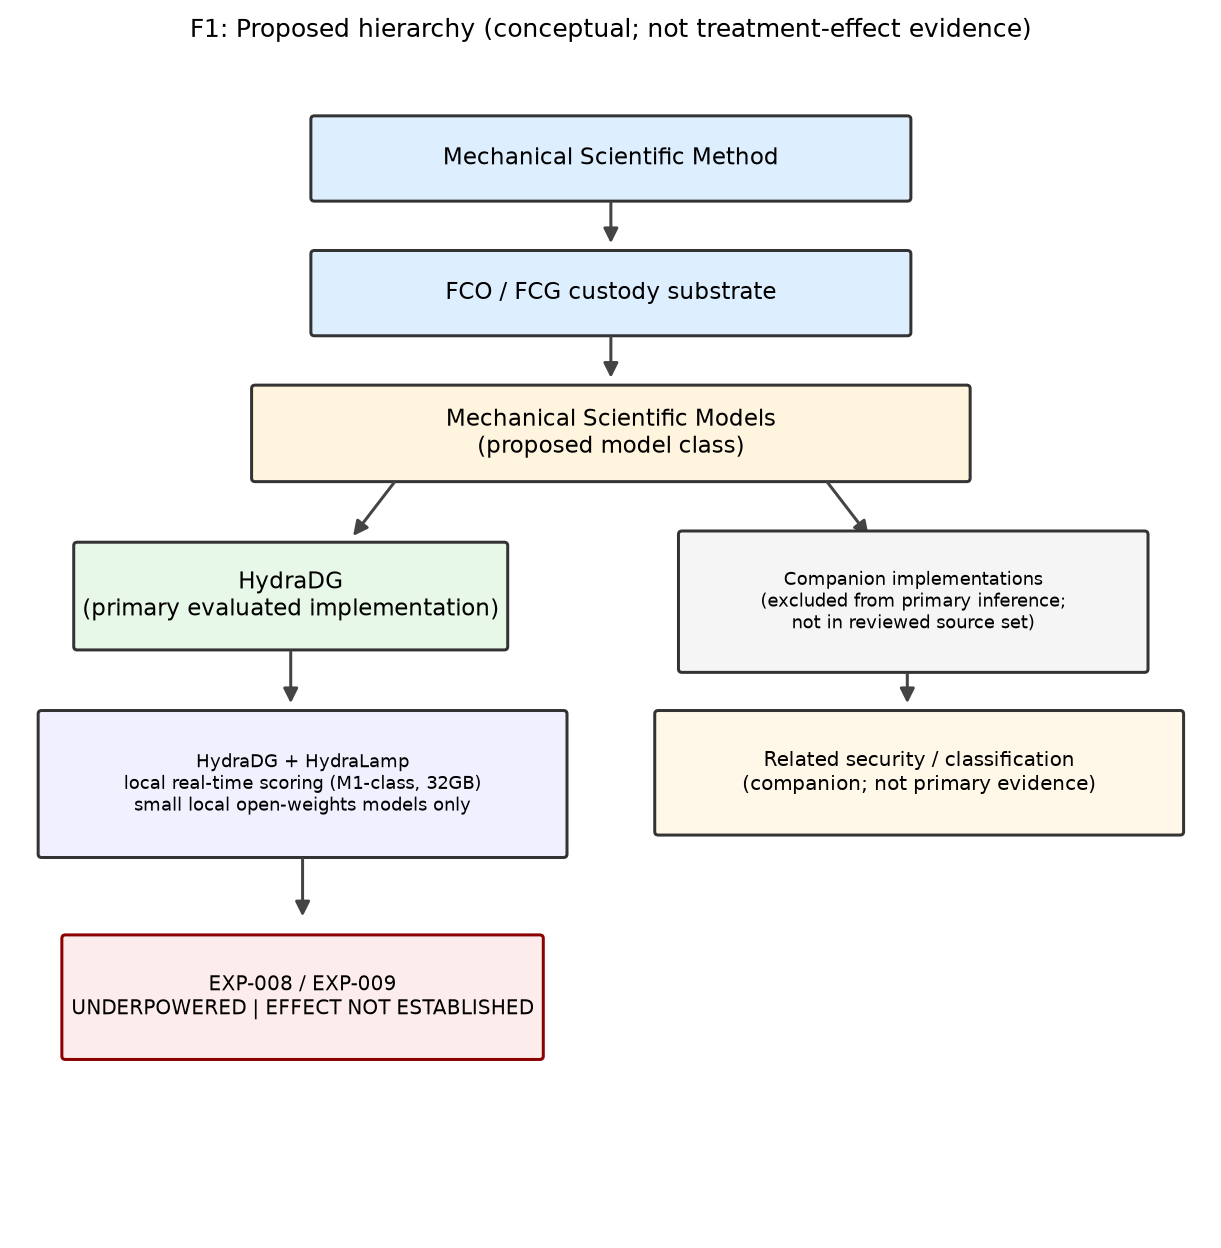
\includegraphics[width=\linewidth]{figures/F1_msm_hierarchy.png}
  \caption{Proposed intellectual hierarchy (conceptual; not empirical effect evidence).
  HydraDG is the primary experimentally evaluated implementation; companion implementations are excluded from primary inference and are not available in the reviewed source set; EXP-008/009 remain \emph{underpowered}.}
  \label{fig:msm-hierarchy}
\end{figure}

\subsection{Custody objects}

An \textbf{FCO} (\emph{Fractal Custody Object}) materializes one bounded transformation: e.g., a model call, scorer pass, or ingest operation.
An \textbf{FCG} (\emph{Fractal Custody Graph}) append records directed edges between FCOs with hash-linked roots \cite{laurie2013ct}.
FCO/FCG provide the custody substrate on which Mechanical Scientific Models record transitions; HydraDG is one implementation that preserves failures, nulls, and malformed outputs in custody (a failure-complete \emph{behavior}, not a redefinition of FCO/FCG).
Claim ceilings (exploratory mechanistic falsification, descriptive only, etc.) are declared at preregistration and enforced at promotion time.

\subsection{Experimental freeze}

Each experiment declares:
\begin{itemize}
  \item frozen case manifest and prompt-contract hashes;
  \item conditions (e.g., flat prose vs.\ structured FCG);
  \item models with expected runtime digests;
  \item primary endpoint and aggregation rule;
  \item explicit gates for confirmatory vs.\ exploratory claims.
\end{itemize}
Execution emits \texttt{START\_RECEIPT}, per-cell raw outputs with prompt/response SHA-256, parser state, and terminal receipts.
Integrity failure (duplicate keys, missing dependencies, silent model substitution) blocks promotion; scientific failure (timeout, abstention, malformed JSON) is retained as terminal evidence.

\subsection{Governed local execution}

Where preregistered, local model calls route through a governed bridge that records selection age, swap posture, and resolved digest.
Direct runtime invocation and governed invocation are separate evidence classes; one is not silently labeled as the other.
EXP-008/009 executed on an Apple Silicon Mac Studio class workstation (32\,GB RAM) with HydraDG scoring and HydraLamp systems-validation receipts on the same host class.

\subsection{Evaluation model policy}

All preregistered scientific endpoints in this submission use small local open-weights models only (\texttt{qwen3:1.7b}, \texttt{qwen2.5-coder:7b}).
Frontier coding agents assisted manuscript preparation only; they did not execute frozen primary scorers or replace verdict-bound cells.

\section{Experimental Setup}

\subsection{Task family}

The IC Failure Learning suite uses synthetic agent-failure vignettes with preregistered endpoints such as E06 (prevents exposure of out-of-vault media).
Cases are drawn from a frozen \texttt{CASES.jsonl} manifest; each case receives multiple replicates per condition.

\subsection{Conditions and models}

\textbf{C0 (FLAT\_PROSE):} failure-handling guidance as unstructured text.\\
\textbf{C1 (STRUCTURED\_FCG):} the same semantic content composed through a frozen FCG retrieval contract.

EXP-008 and EXP-009 used local models \texttt{qwen3:1.7b} and \texttt{qwen2.5-coder:7b} under identical case and scorer contracts on private M1-class hardware (32\,GB RAM).
Thinking/reasoning modes were held consistent with preregistration.
Primary aggregation: majority of three replicates per case, then paired comparison at the model-stratum level.
The preregistered confirmatory aggregation operates at the paired model-stratum level, yielding \texttt{n\_paired}$=2$; the 300 raw execution cells are pre-aggregation replicates and do not constitute 300 independent confirmatory treatment pairs.
Historical LongMemEval track-03 retrieval ablations under the same local-only policy are excluded from primary inference and are not promoted here.

\subsection{AI and agent methodology disclosure}

Frontier coding agents assisted with repository tooling and manuscript preparation; they are not listed as authors.
All scientific endpoints come from preregistered local model executions with hashed prompts and responses.
Routine editing does not constitute a reported experimental intervention.

\subsection{Power and claim gates}

E06 endpoints are known limited-power under the frozen case set.
Confirmatory ordering claims require preregistered discordant pairs; exploratory secondary statistics are quarantined from primary promotion.


\begin{figure}[t]
  \centering
  
\includegraphics[width=\linewidth]{figures/F2.png}
  \caption{Primary EXP-008/009 outcomes from frozen verdict JSON: top panels show attrition (raw $\rightarrow$ paired); bottom panels show terminal failure rates (malformed, abstain, unknown). H0 reference shown; UNDERPOWERED --- effect not established (not proof of null).}
  \label{fig:primary-hypothesis}
\end{figure}

\section{Results}

Table~\ref{tab:terminal} summarizes terminal verdicts for preregistered studies.
Figure~\ref{fig:primary-hypothesis} decomposes the same receipts into attrition counts and \texttt{data\_quality} rates ($n_{\mathrm{raw}}=300$ per study).
Both experiments executed the full raw matrix with complete custody append.

\begin{table}[t]
  \centering
  \caption{Terminal preregistered studies (HydraDG IC Failure Learning). \emph{Underpowered} denotes insufficient paired evidence for confirmatory promotion, not proof of null effect.}
  \label{tab:terminal}
  \begin{tabular}{llll}
    \toprule
    Study & Primary verdict & Raw cells & Valid parse rate \\
    \midrule
    EXP-008 & UNDERPOWERED & 300 & 0.907 \\
    EXP-009 & UNDERPOWERED & 300 & 0.883 \\
    \bottomrule
  \end{tabular}
\end{table}

\textbf{EXP-008.} Structured FCG retrieval did not yield promotable confirmatory evidence on E06 under the frozen design ($n=2$ paired cases per model stratum at aggregation scope). Non-zero malformed and abstention rates are preserved in custody.

\textbf{EXP-009.} Primary verdict remains UNDERPOWERED for confirmatory E06 ordering. An exploratory secondary pattern was recorded as directionally positive at the descriptive layer only; it is \textbf{not promoted} to a causal claim.

\textbf{Stage-2 baseline.} Prior IC Failure Learning stage-2 execution (414 scored rows across two models) established that failure-learning behavior improvement was not established under that frozen design, providing historical context for the structured-retrieval falsification lane.
Historical LongMemEval track-03 lanes (local open-weights models, frozen primary scorer) are retained for internal audit only; they were not executed with frontier models and do not upgrade primary EXP-008/009 claims.


\begin{figure}[t]
  \centering
  
\includegraphics[width=\linewidth]{figures/F6.png}
  \caption{HydraLamp perturbation test matrix (systems robustness only; not treatment-effect evidence).}
\end{figure}

\subsection{Failure-preserving systems validation}

The preregistered retrieval experiments above test whether structured context improves a frozen endpoint.
A separate systems-validation suite asks a different question: does the custody mechanism preserve integrity under perturbation, tampering, concurrency, replay, and external execution failure?
Table~\ref{tab:systems} summarizes source-verified outcomes from a frozen HydraLamp perturbation matrix; these results evaluate custody mechanics and do \textbf{not} constitute evidence that structured FCG context improves the EXP-008/009 endpoint.

\begin{table}[t]
  \centering
  \caption{Systems-validation outcomes (custody mechanics only; not treatment-effect evidence).}
  \label{tab:systems}
  \begin{tabular}{lll}
    \toprule
    Validation & Scope & Outcome \\
    \midrule
    Perturbation matrix & 100 cells & 100/100 chain verification \\
    Synthetic tamper suite & 8 modes & 8/8 detected \\
    Concurrent execution & 10 runs & PASS (10 unique run IDs) \\
    Replay/restart recovery & 44 events & PASS \\
    Live provider ladder & R0--R6 & Bounded external failure preserved \\
    \bottomrule
  \end{tabular}
\end{table}

The tamper suite used synthetic cases only (not real security incidents).
In a live provider repair ladder, earlier infrastructure gates passed before a structured call hit an external quota limit; the failure remained a terminal auditable state rather than being erased or substituted.
The same custody primitives have been instantiated in sibling systems for local-model orchestration, deterministic scientific-document atomization, offline anomaly detection, bounded bioinformatics, substrate generation, and operator-facing scientific workflow monitoring; these implementations motivate transfer studies but do not provide additional evidence for the treatment effect reported here.

\section{Discussion}

The principal contribution of this submission is not evidence that structured FCG retrieval improves failure prevention.
EXP-008 and EXP-009 remain \emph{underpowered}; the empirical retrieval effect on the preregistered E06 endpoint is \emph{not established}.
The broader methodological proposition is that scientific computational models can expose their evidence-state transitions mechanically---through governed receipts, explicit claim ceilings, and preserved terminal states---so that null, failure, and blocked outcomes remain part of model state rather than disappearing from the public record.

HydraDG demonstrates bounded custody and systems-validation behavior under that contract: failures are first-class, hashes are mandatory, and claim ceilings block over-interpretation.
HydraLamp perturbation, tamper, concurrency, and replay results (Table~\ref{tab:systems}) evaluate custody mechanics only.
Companion implementation lineages are admitted as related implementations excluded from primary inference; their run receipts are not available in the reviewed source set for this submission.
The EXP-008/009 underpowered terminations bound what cannot yet be claimed while preserving malformed and timeout cells for audit.

\subsection{Limitations}
\label{sec:limitations}

Limitations include bounded case replication, deliberate local-only small-model lanes in the reported matrix (no frontier API substitution), and absence of runtime-equivalent successor replication in primary results.
Execution hardware was constrained to M1-class Apple Silicon with 32\,GB RAM; results do not establish performance on datacenter GPU fleets or frontier-model endpoints.
A preregistered Qwen~3.8 successor lane exists but is non-terminal and omitted from primary results.
Whole-project hierarchical atomization (SeedGraph v1a validation) ran for multiple days but was interrupted during final Parquet serialization without a terminal build receipt; partial node/edge artifacts are not readback-safe, so terminal whole-corpus atomization is not established in this submission.
Biological, protein-structure, and cellular perturbation applications of the custody framework remain future validation targets, not demonstrated generalizations of the agent-context results here.

\subsection{Future directions}

\textbf{Agent systems.} Larger successor replications, governed multi-agent handoffs, selective replay, and resource-aware custody gates under preregistered manifests.

\textbf{Structured retrieval at scale.} Checkpointed ingest and transactionally durable atomization so long hierarchy builds can resume from batch boundaries rather than materializing the entire graph at finalization.

\textbf{Cross-project federation.} Project-local FCG roots with explicit cross-project references and no automatic evidence admission between repositories.

\textbf{Cryptographic custody.} Authorized signatures and MMR commitments where policy permits; hashes remain identity commitments unless a verified signing operation occurred.

All directions above are \emph{planned} unless independently measured; they do not extend the EXP-008/009 empirical claims.

\section{Conclusion}

We proposed the term \emph{Mechanical Scientific Model} for a computational model class whose governed state transitions expose evidence, separate deterministic from probabilistic outputs, preserve failure-complete terminal states, and bind explicit claim ceilings with forward and reverse traceability.
FCO/FCG provide the custody substrate; HydraDG is one implementation examined here under that proposal.
Two preregistered HydraDG studies (EXP-008, EXP-009) closed as \emph{underpowered}, demonstrating bounded custody and systems behavior while withholding confirmatory promotion of structured retrieval effects on failure-prevention endpoints.
We recommend explicit Mechanical Scientific Method discipline---custody receipts, claim ceilings, and terminal-state preservation---as baseline infrastructure for NewInML-style agent evaluations, without claiming that structured retrieval efficacy has been established.

\begin{thebibliography}{19}

\bibitem{lewis2020rag}
P.~Lewis, E.~Perez, A.~Piktus, et al.
\newblock Retrieval-augmented generation for knowledge-intensive {NLP} tasks.
\newblock In \emph{NeurIPS}, 2020.
\newblock arXiv:2005.11401.

\bibitem{liu2023agentbench}
Y.~Liu et al.
\newblock {AgentBench}: Evaluating {LLMs} as agents.
\newblock arXiv:2308.03688, 2023.

\bibitem{zhou2023webarena}
S.~Zhou et al.
\newblock {WebArena}: A realistic web environment for building autonomous agents.
\newblock arXiv:2307.13854, 2023.

\bibitem{edge2024graphrag}
D.~Edge et al.
\newblock From local to global: A graph {RAG} approach to query-focused summarization.
\newblock Microsoft Research, 2024.
\newblock arXiv:2404.16130.

\bibitem{nosek2018prereg}
B.~A. Nosek, C.~R. Ebersole, A.~C. DeHaven, and D.~T. Mellor.
\newblock The preregistration revolution.
\newblock \emph{PNAS}, 115(11):2600--2606, 2018.

\bibitem{wilkinson2016fair}
M.~D. Wilkinson et al.
\newblock The {FAIR} guiding principles for scientific data management and stewardship.
\newblock \emph{Scientific Data}, 3:160018, 2016.

\bibitem{groth2010nano}
P.~Groth, A.~Gibson, and J.~Velterop.
\newblock The anatomy of a nanopublication.
\newblock \emph{Information Services \& Use}, 30(1--2):51--56, 2010.

\bibitem{prereg2026}
Anonymous. (2026). HydraDG IC Failure Learning preregistrations EXP-008 and EXP-009. Internal frozen artifacts; anonymized submission.

\bibitem{stage2}
Anonymous. (2026). IC Failure Learning Stage-2 closeout receipt. Internal frozen artifacts; anonymized submission.

\bibitem{neurips2026}
NeurIPS. (2026). New in Machine Learning (NewInML) workshop call for papers. Non-archival workshop track.

\bibitem{laurie2013ct}
B.~Laurie, A.~Langley, and E.~Kasper.
\newblock Certificate Transparency.
\newblock RFC~6962, IETF, June 2013.

\bibitem{lebo2013provo}
T.~Lebo et al.
\newblock PROV-O: The PROV Ontology.
\newblock W3C Recommendation, 2013.

\bibitem{khan2019cwlprov}
F.~Z. Khan et al.
\newblock Sharing interoperable workflow provenance: A review of best practices and their practical application in {CWLProv}.
\newblock \emph{GigaScience}, 8(11):giz095, 2019.
\newblock DOI:10.1093/gigascience/giz095.

\bibitem{karl2024negative}
F.~Karl, L.~M. Kemeter, G.~Dax, and P.~Sierak.
\newblock Position: Embracing negative results in machine learning.
\newblock In \emph{ICML}, PMLR 235:23256--23265, 2024.
\newblock arXiv:2406.03980.

\bibitem{wang2026agentprovenance}
Y.~Wang et al.
\newblock From Agent Traces to Trust: Evidence Tracing and Execution Provenance in {LLM} Agents.
\newblock arXiv:2606.04990, 2026.

\bibitem{kuhn2014trusty}
T.~Kuhn and M.~Dumontier.
\newblock Trusty {URIs}: verifiable, immutable digital artifacts.
\newblock In \emph{ESWC}, 2014.

\bibitem{walters2023fabrication}
W.~H. Walters and E.~I. Wilder.
\newblock Fabrication and errors in bibliographic citations generated by {ChatGPT}.
\newblock \emph{Scientific Reports}, 13:14045, 2023.

\bibitem{leo2024rocrote}
S.~Leo et al.
\newblock Recording provenance of workflow runs with {RO-Crate}.
\newblock \emph{PLOS ONE}, 19(9):e0309210, 2024.

\end{thebibliography}

\ifincludeappendix
\appendix
\section{Full EXP-008 / EXP-009 statistical audit}
\label{app:exp-stats}
Table~\ref{tab:app_exp_stats} records terminal verdicts with parse rates reverse-traced to frozen verdict JSON receipts. $p$-values remain \emph{not informative} under the preregistered underpowered design.

\begin{table}[h]
  \centering
  \caption{Terminal preregistered study audit (appendix).}
  \label{tab:app_exp_stats}
  \begin{tabular}{llll}
    \toprule
    Study & Verdict & Raw cells & Valid parse rate \\
    \midrule
    EXP-008 & UNDERPOWERED & 300 & 0.907 \\
    EXP-009 & UNDERPOWERED & 300 & 0.883 \\
    \bottomrule
  \end{tabular}
\end{table}

\section{Stage-2 M0/M1/M2 baseline}
\label{app:stage2}
Stage-2 IC Failure Learning execution (414 scored rows across two models) closed as \texttt{FAILURE\_LEARNING\_BEHAVIOR\_IMPROVEMENT\_NOT\_ESTABLISHED}; descriptive only.

\section{HydraLamp systems-validation matrix}
\label{app:systems}
See Table~\ref{tab:app_systems} for custody-mechanics outcomes (not treatment-effect evidence).

\begin{table}[h]
  \centering
  \caption{Systems-validation matrix (appendix).}
  \label{tab:app_systems}
  \begin{tabular}{lll}
    \toprule
    Validation & Scope & Outcome \\
    \midrule
    Perturbation matrix & 100 cells & 100/100 chain verification \\
    Synthetic tamper suite & 8 modes & 8/8 detected \\
    Concurrent execution & 10 runs & PASS (10 unique run IDs) \\
    Replay/restart recovery & 44 events & PASS \\
    Live provider ladder & R0--R6 & Bounded external failure preserved \\
    \bottomrule
  \end{tabular}
\end{table}

\section{Deterministic verification and tooling}
\label{app:tooling}
Figure~\ref{fig:custody-pipeline} and \texttt{DETERMINISTIC\_AUDIT\_TOOLING\_LEDGER.jsonl} document the custody verification pipeline with frozen script SHA-256 and R1/R2/R3 roots.

\begin{figure}[ht]
  \centering
  \fbox{\begin{minipage}{0.92\linewidth}
  \small
  Source bytes $\rightarrow$ SHA-256 $\rightarrow$ Atom $\rightarrow$ ResultAtom $\rightarrow$ Claim/Table $\rightarrow$ FCG delta $\rightarrow$ exact-SHA verification
  \end{minipage}}
  \caption{FIG-001: governed custody pipeline from source bytes to exact-SHA verification (structured data; self-generated).}
  \label{fig:custody-pipeline}
\end{figure}

\section{Citation and reference custody}
\label{app:citations}
Portfolio recovery bounded 185 occurrences to unique identities; only proposition-backed references are admitted. Citation fabrication literature informs desk-rejection risk \cite{kuhn2014trusty}, \cite{walters2023fabrication}, \cite{khan2019cwlprov}, \cite{leo2024rocrote}, \cite{lebo2013provo}.

\section{Requirement, template, and deadline drift}
\label{app:requirements}
The NewInML workshop submission form requests a CC~BY~4.0 article license for this non-archival track; OpenReview platform terms govern platform use separately from article and repository licenses. Repository code remains Apache-2.0 (separate layer).

\section{Prior-art comparison matrix}
\label{app:priorart}
Related-work boundaries include PROV-O, CWLProv, and Workflow Run RO-Crate \cite{kuhn2014trusty}, \cite{walters2023fabrication}, \cite{khan2019cwlprov}, \cite{leo2024rocrote}, \cite{lebo2013provo}. Prior-art search responses remain \emph{DISCOVERY\_ONLY}; not promoted to verified empirical novelty proof.

\section{SeedGraph / FCO / FCG custody audit}
\label{app:seedgraph}
\texttt{TOTAL\_VERIFIED\_INGEST\_COMPLETE=NO} with verified coverage 31.55\% (307/973).

\section{Planned and nonterminal lanes}
\label{app:planned}
GPU SGLang canary, Q38 XENV, and full verified ingest remain nonterminal.
All appendix citations resolve through the single main-text bibliography authority.

\fi

\newpage
\vspace*{-0.4em}
{\scriptsize\noindent FCO-CUSTODY: \texttt{1a6b0a967da41e5b} \quad HASH: SHA-256 \quad TREE: \texttt{fco\_train.custody.merkle\_root.v3} \quad KEY-ID: PENDING\\
CONTENT-ROOT: \texttt{1a6b0a967da41e5b619ec449ab0cdbb9\allowbreak 14797321661e7ee25f8b87f2521df94d}}
\vspace{0.4em}

\input{checklist.tex}

\end{document}
